
\documentclass[12pt]{report}
\usepackage[utf8]{inputenc}
\usepackage{graphicx}
\usepackage{hyperref}
\graphicspath{ {./Poze/} }
\usepackage{setspace}
\usepackage{color, soul}

\usepackage[margin=1in]{geometry}
% \usepackage{txfonts}
\usepackage{listings}
\usepackage{cleveref}
\usepackage{xcolor}
\renewcommand{\lstlistingname}{Code}
\renewcommand{\lstlistlistingname}{List of Code}

\lstdefinestyle{chstyle}{%
backgroundcolor=\color{gray!12},
basicstyle=\ttfamily\small,
commentstyle=\color{green!60!black},
keywordstyle=\color{magenta},
stringstyle=\color{blue!50!red},
showstringspaces=false,
%captionpos=b,
numbers=left,
numberstyle=\footnotesize\color{gray},
numbersep=10pt,
%stepnumber=2,
tabsize=2,
frame=L,
framerule=1pt,
rulecolor=\color{red},
breaklines=true,
inputpath=code
}

\renewcommand{\baselinestretch}{1.15} 
\renewcommand{\contentsname}{Cuprins}

\usepackage{titlesec}

\titlespacing{\chapter}{0pt}{*-10}{*5}

\titleformat{\chapter}[display]
  {\normalfont\bfseries}{}{0pt}{\Huge}

\title{Proiect 1 - Grafică pe Calculator\\
\Large - Depășire între 2 dreptunghiuri -}
\date{- 10 Noiembrie 2022 -}
\author{Linte Robert Ovidiu\\ Popescu Paullo Robertto Karloss\\
\large Grupa 331\\\\
\large Conf. Dr. Stupariu Mihai-Sorin
}

\hypersetup{
    colorlinks,
    citecolor=black,
    filecolor=black,
    linkcolor=black,
    urlcolor=black
}

\begin{document}
    \maketitle
    \tableofcontents
    \chapter{Introducere}
    \section{Modul de organizare al echipei}
    Echipa noastră:
    \begin{itemize}
        \item Linte Robert Ovidiu
        \item Popescu Paullo Robertto Karloss
    \end{itemize}
    Se va specifica \textbf{numele} membrului care a \textbf{contribuit} la realizarea fiecărei \emph{etape}.
    \section{Obiectivele proiectului}
    Simularea unei "depășiri":
    \begin{itemize}
        \item O mașină (un dreptunghi) se deplasează pe o șosea uniform (print translație)
        \item O altă mașină (alt dreptunghi) vine din spate (tot prin translații)
        \item La un moment dat a doua mașină intră în depășire
        \item A doua mașină trece în fața primei mașini
        \item Se afișează la final câștigătorul "cursei"
    \end{itemize}
    Aprofundarea cunoștințelor în OpenGL prin:
    \begin{itemize}
        \item Utilizarea translațiilor
        \item Desenarea obiectelor
        \item Utilizarea culorilor
    \end{itemize}

    \section{Vizionarea proiectului}
    Puteți viziona \emph{demo-ul} proiectului \href{https://youtu.be/itgOAlJtbVY}{\textbf{\textit{\hl{aici}}}}, iar \emph{repository-ul} de pe Github \href{https://github.com/linterobert/Proiect-Grafica}{\textbf{\textit{\hl{aici}}}}.

    \newpage
    \chapter{Desenarea obiectelor}
    Această etapă a fost realizată de \emph{\textbf{Popescu Paullo Robertto Karloss}}.
    \section{Prezentarea tablei de joc}
    Tabla de joc conține:
    \begin{itemize}
        \item Șoseua propiu-zisă
        \item O linie punctată pe post de marcaj rutier
        \item Două mașini de culori diferite (prima roșie, a doua albastră) care au forma unor dreptunghiuri
        \item Iarbă pe marginea șoselei
        \item Un text la finalul șoselei cu mesajul "FINISH", pentru scoate în evidență câștigătorul "cursei"
    \end{itemize}
    \begin{center}
        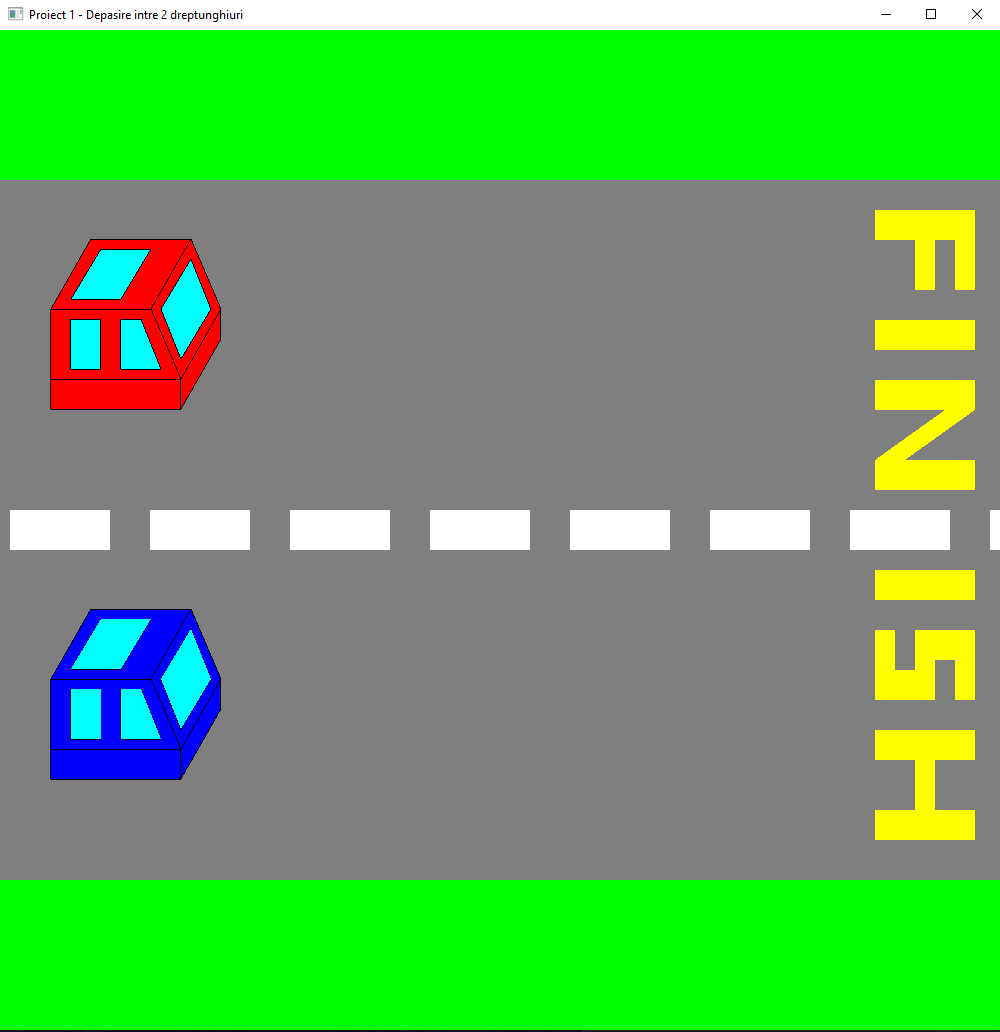
\includegraphics[width=15cm, height=8.7cm]{Poza1.png}
    \end{center}
    \begin{center}
        Figura 2.1: Tabla de joc
    \end{center}

    \section{Cum a fost construită tabla de joc}
    Pentru a construi tabla de joc am creat un background (un dreptunghi) de culoare verde.
    Peste acesta am adăugat șoseaua (un dreptunghi de culoare gri).
    După care, în interiorul șoselei am creat două dreptunghiuri, unul roșu si unul albastru, pe post de mașini, 
    drepunghiuri albe pe post de linie punctată (marcaj rutier din legislație) și alte dreptunghirui de culoare galbenă pentru a scrie mesajul \emph{"FINISH"}.


    \section{Cod sursă}
    \lstinputlisting[language=C++, style=chstyle, label=cpp-sample]{puncte.cpp}
    \begin{center}
        Figura 2.1: Crearea punctelor și a culorilor pentru Tabla de joc
    \end{center}
    
    \newpage
    \lstinputlisting[language=C++, style=chstyle, label=cpp-sample]{Desen.cpp}

    \begin{center}
        Figura 2.2:Cod OpenGL pentru Tabla de joc
    \end{center}

    \lstinputlisting[language=C++, style=chstyle, label=cpp-sample]{Desen2.cpp}

    \begin{center}
        Figura 2.3: Cod OpenGL pentru Tabla de joc
    \end{center}

    \lstinputlisting[language=C++, style=chstyle, label=cpp-sample]{Desen3.cpp}

    \begin{center}
        Figura 2.4: Cod OpenGL pentru Tabla de joc
    \end{center}

    \lstinputlisting[language=C++, style=chstyle, label=cpp-sample]{Desen4.cpp}

    \begin{center}
        Figura 2.5: Cod OpenGL pentru Tabla de joc
    \end{center}

    \newpage
    \chapter{Adăugarea translațiilor}
    Această etapă a fost realizată de \emph{\textbf{Linte Robert Ovidiu}}.
    \section{Prezentarea Translației 1}
    Dreptunghiul roșu pleacă cu o viteză inițială mai mică decât a dreptunghiului albastru.
    \begin{center}
        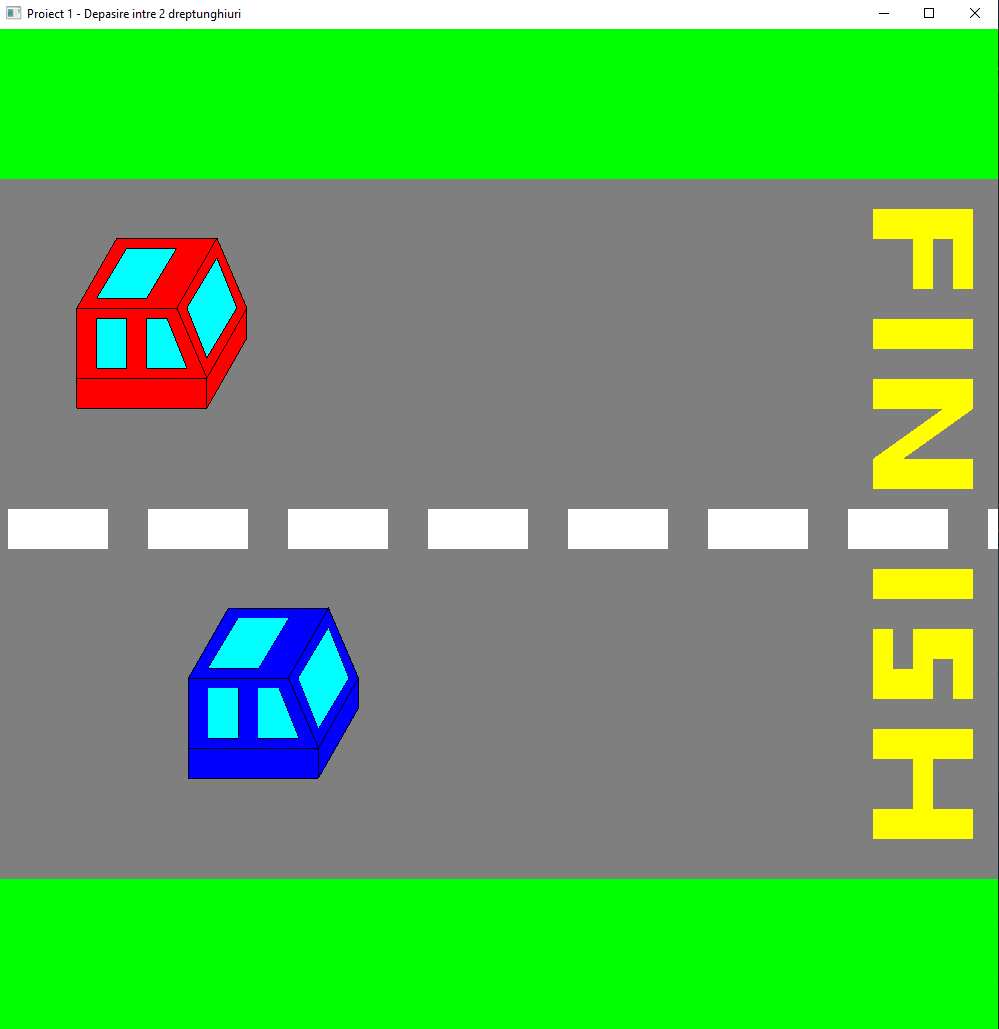
\includegraphics[width=15cm, height=8.7cm]{Poza3.png}
    \end{center}
    \begin{center}
        Figura 3.1.1: Deplasarea inițială a dreptunghiurilor
    \end{center}

    \subsection{Cod sursă}
    % \begin{center}
    %     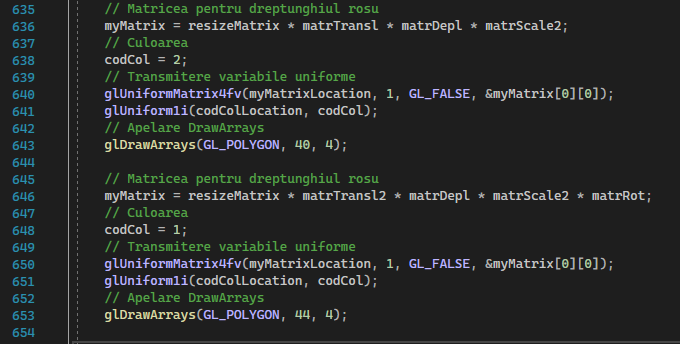
\includegraphics[width=15cm, height=8.3cm]{Poza4.png}
    % \end{center}
    \lstinputlisting[language=C++, style=chstyle, label=cpp-sample]{first.cpp}
    \begin{center}
        Figura 3.1.2: Cod OpenGL pentru prima translație
    \end{center}

    % \begin{center}
    %     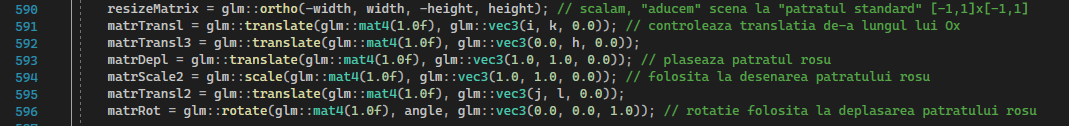
\includegraphics[width=15cm, height=2.2cm]{Poza5.png}
    % \end{center}
    \lstinputlisting[language=C++, style=chstyle, label=cpp-sample]{primaTranslatie2.cpp}
    \begin{center}
        Figura 3.1.3: Cod OpenGL pentru prima translație
    \end{center}

    % \begin{center}
    %     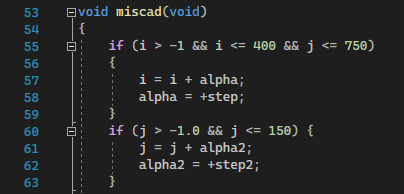
\includegraphics[width=8cm, height=3.4cm]{Poza6.png}
    % \end{center}
    \lstinputlisting[language=C++, style=chstyle, label=cpp-sample]{primaTranslatie.cpp}
    \begin{center}
        Figura 3.1.4: Cod OpenGL pentru prima translație
    \end{center}

    \section{Prezentarea Translației 2}
    În momentul în care dreptunghiul albastru, îl depășeste total pe cel roșu, începe procesul de depășire \emph{(se aplică
    o rotație de 0.5 pe dreptunghiul albastru cât și o translație pe diagonală, iar în final se aplică o rotație
    inversă pentru a-l aduce pe poziția inițială, i.e. paralel cu axa Ox)}.
    \begin{center}
        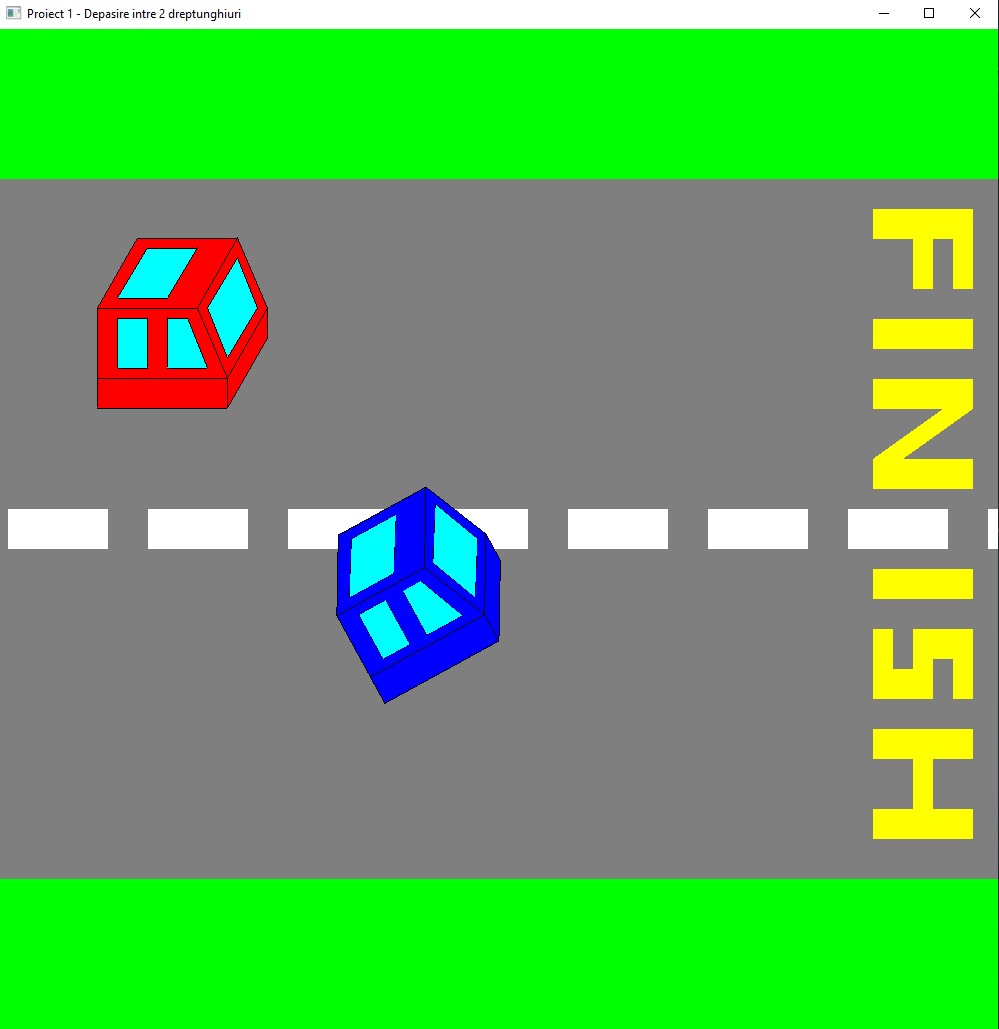
\includegraphics[width=15cm, height=8.7cm]{Poza8.png}
    \end{center}
    \begin{center}
        Figura 3.2.1: Depășire dreptunghi roșu
    \end{center}

    \begin{center}
        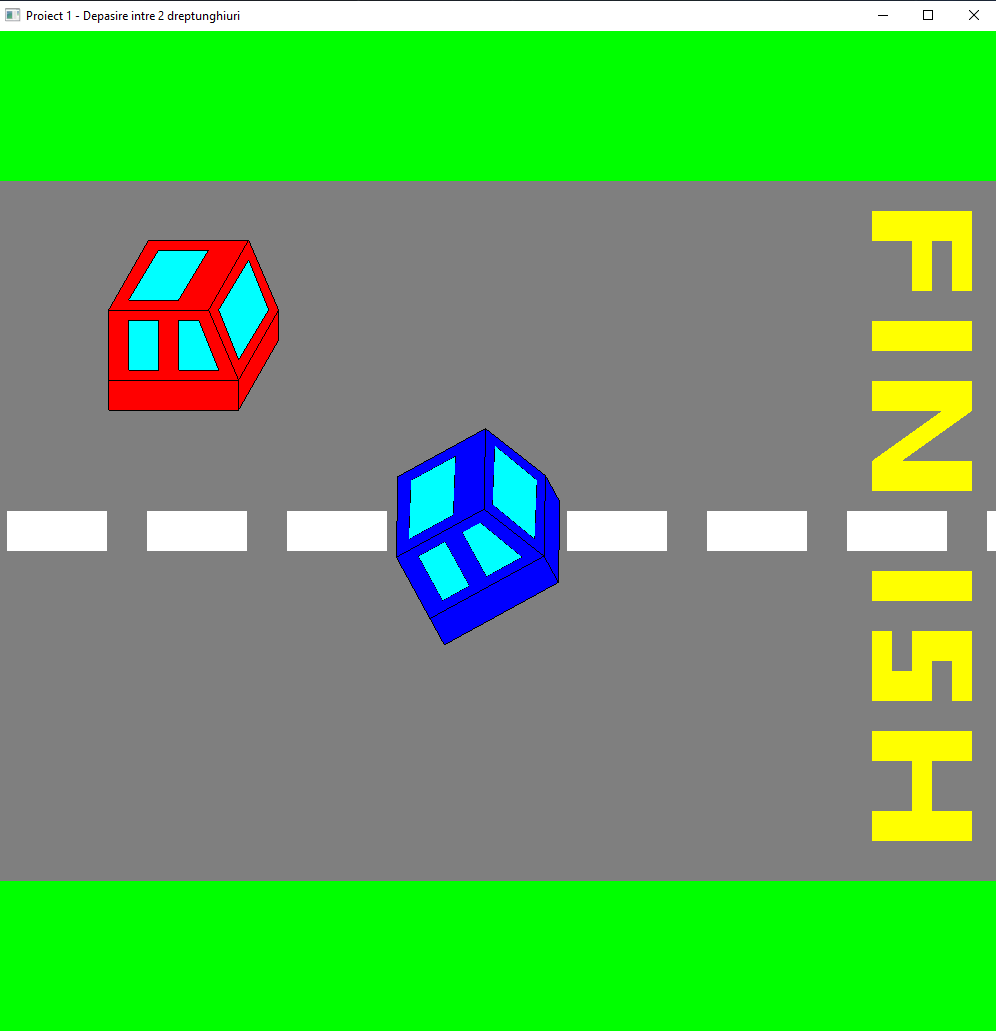
\includegraphics[width=15cm, height=8.7cm]{Poza9.png}
    \end{center}
    \begin{center}
        Figura 3.2.2: Depășire dreptunghi roșu
    \end{center}


    \subsection{Cod sursă}
    % \begin{center}
    %     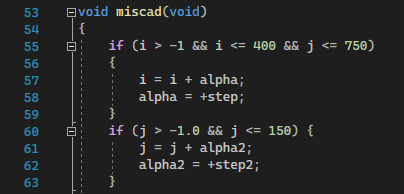
\includegraphics[width=9cm, height=3.5cm]{Poza6.png}
    % \end{center}
    \lstinputlisting[language=C++, style=chstyle, label=cpp-sample]{depasire.cpp}
    \begin{center}
        Figura 3.2.3: Cod OpenGL pentru a doua translație
    \end{center}

    \newpage
    \section{Prezentarea Translației 3}
    După translația 2, dreptunghiul albastru accelerează până trece linia de \emph{"FINISH"}.
    \begin{center}
        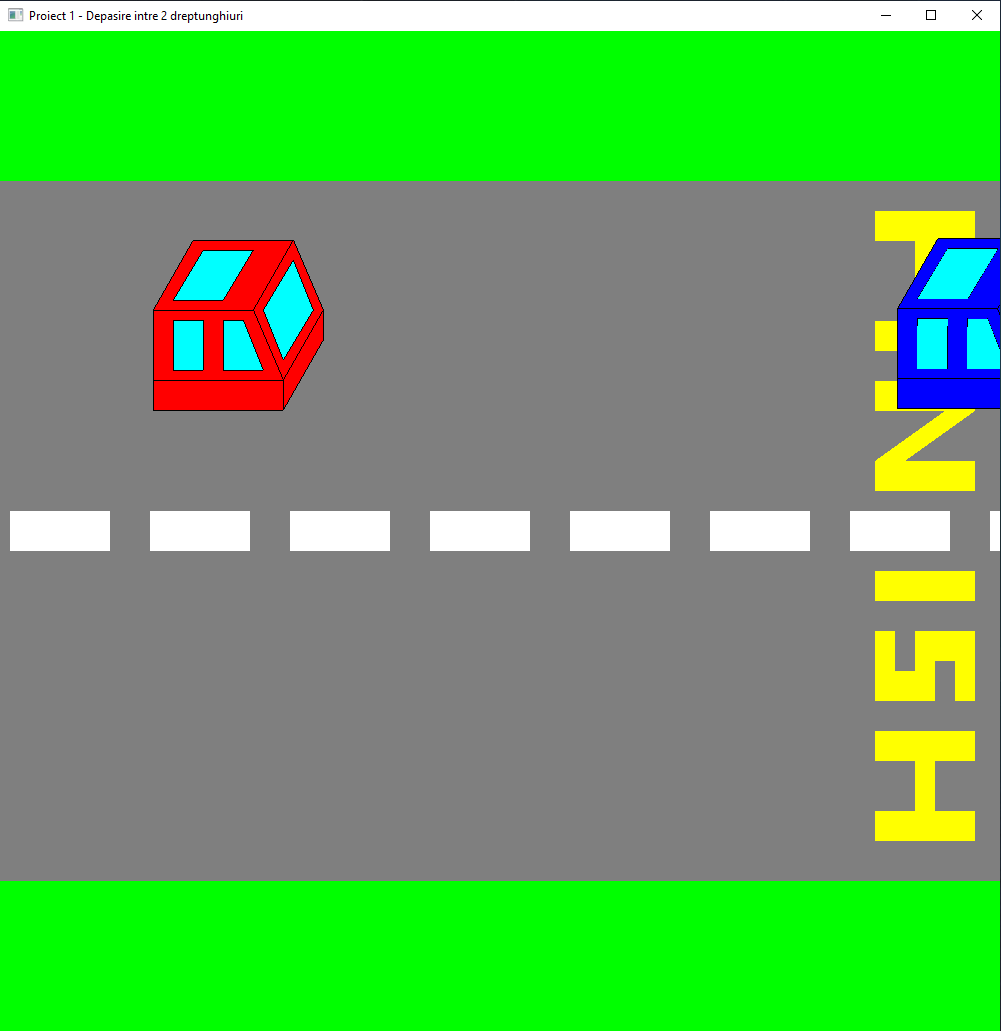
\includegraphics[width=15cm, height=8.7cm]{Poza10.png}
    \end{center}
    \begin{center}
        Figura 3.2.1: Accelerare dreptunghi albastru
    \end{center}

    \subsection{Cod sursă}
    % \begin{center}
    %     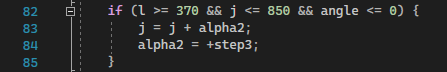
\includegraphics[width=10cm, height=2cm]{Poza11.png}
    % \end{center}
    \lstinputlisting[language=C++, style=chstyle, label=cpp-sample]{litereAscunse.cpp}
    \begin{center}
        Figura 3.3.1: Cod OpenGL pentru a treia translație
    \end{center}

    \chapter{Afișarea câștigătorului}
    \section{Prezentarea înainte de translația finală}
    Literele sunt inițial puse în afara ecranului \emph{(nu sunt vizibile în tabla de joc)}.
    \subsection{Cod sursă}
    % \begin{center}
    %     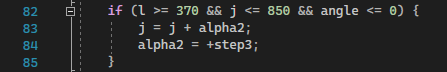
\includegraphics[width=10cm, height=2cm]{Poza11.png}
    % \end{center}
    \lstinputlisting[language=C++, style=chstyle, label=cpp-sample]{litereAscunse2.cpp}
    \begin{center}
        Figura 4.1.1: Cod OpenGL pentru literele ascunse
    \end{center}

    Această etapă a fost realizată de \emph{\textbf{Popescu Paullo Robertto Karloss}}.

    \section{Prezentare după translație}
    După ce dreptunghiul albastru reusește să treacă linia de \emph{"FINISH"}, sunt translatate literele în zona de sus a tablei de joc.
    \begin{center}
        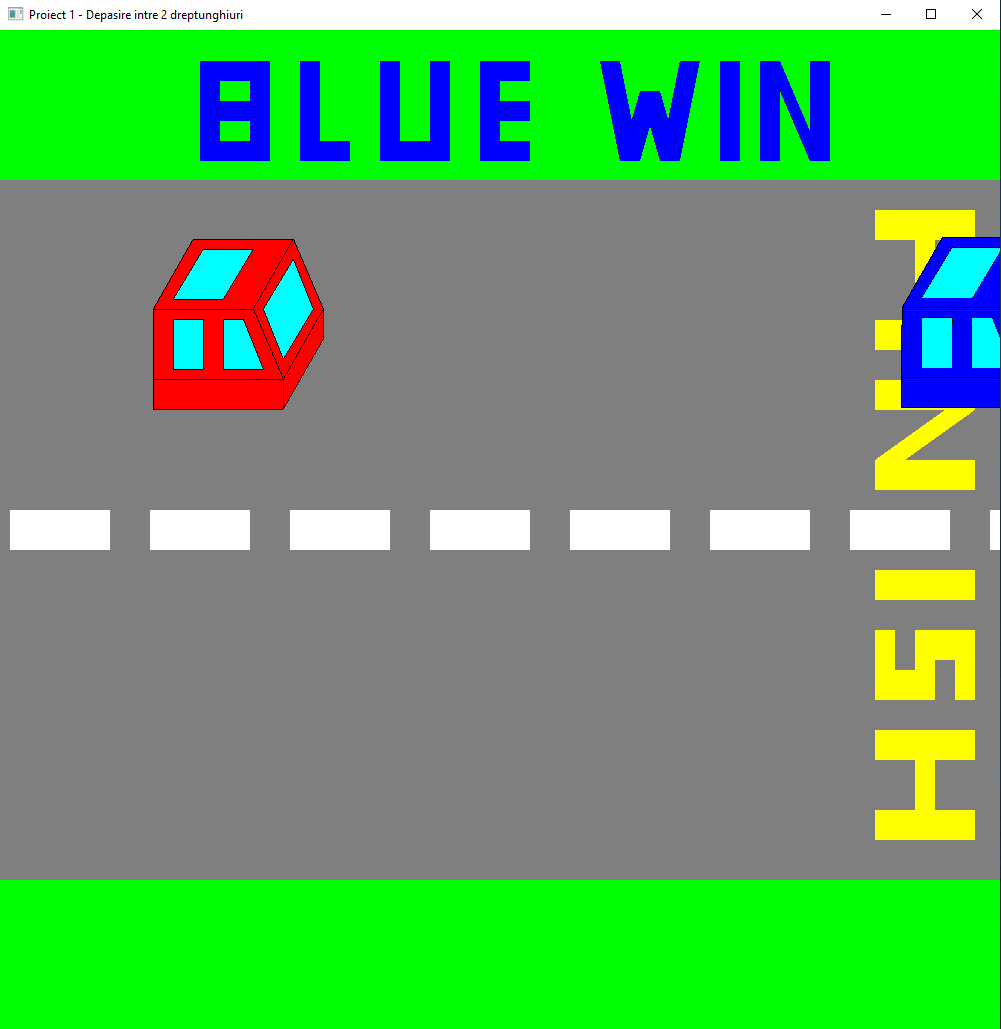
\includegraphics[width=13cm, height=7.25cm]{Poza12.png}
    \end{center}
    \begin{center}
        Figura 4.1.1: Afișarea câștigătorului
    \end{center}

    \subsection{Cod sursă}
    % \begin{center}
    %     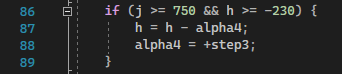
\includegraphics[width=10cm, height=1.8cm]{Poza13.png}
    % \end{center}
    \lstinputlisting[language=C++, style=chstyle, label=cpp-sample]{translatieFinala.cpp}
    \begin{center}
        Figura 4.1.1: Cod OpenGL pentru translația finală
    \end{center}

    Această etapă a fost realizată de \emph{\textbf{Linte Robert Ovidiu}}.

    \newpage
    \chapter{Codul Sursă Complet}
    Codul îl puteți găsi în fișierul \href{https://github.com/linterobert/Proiect-Grafica/blob/master/GraphicsProject/GraphicsProject/proiectGrafica.cpp}{\textbf{\emph{\hl{proiectGrafica.cpp}}}} sau atașat mai jos.
    \lstinputlisting[language=C++, style=chstyle, label=cpp-sample]{proiectGrafica.cpp}
    
    \newpage
    \chapter{Codul pentru Shader}
    Codul îl puteți găsi în fișierul \href{https://github.com/linterobert/Proiect-Grafica/blob/master/GraphicsProject/GraphicsProject/03_02_Shader.frag}{\textbf{\emph{\hl{03\_02\_Shader.frag}}}} sau atașat mai jos.
    \lstinputlisting[language=C++, style=chstyle, label=cpp-sample]{03_02_Shader.frag}
    
    \newpage
    \chapter{Referințe}
    \begin{itemize}
        \item Fișierul \emph{03\_02\_animatie\_new.cpp} din \emph{Laborator 3}.
        \item \emph{Materialele din Curs}.
    \end{itemize}

\end{document}